% Options for packages loaded elsewhere
\PassOptionsToPackage{unicode}{hyperref}
\PassOptionsToPackage{hyphens}{url}
\PassOptionsToPackage{dvipsnames,svgnames,x11names}{xcolor}
%
\documentclass[
  11pt,
]{article}

\usepackage{amsmath,amssymb}
\usepackage{setspace}
\usepackage{iftex}
\ifPDFTeX
  \usepackage[T1]{fontenc}
  \usepackage[utf8]{inputenc}
  \usepackage{textcomp} % provide euro and other symbols
\else % if luatex or xetex
  \usepackage{unicode-math}
  \defaultfontfeatures{Scale=MatchLowercase}
  \defaultfontfeatures[\rmfamily]{Ligatures=TeX,Scale=1}
\fi
\usepackage{lmodern}
\ifPDFTeX\else  
    % xetex/luatex font selection
    \setmainfont[]{Arial}
    \setsansfont[]{Arial}
    \setmonofont[]{Courier New}
\fi
% Use upquote if available, for straight quotes in verbatim environments
\IfFileExists{upquote.sty}{\usepackage{upquote}}{}
\IfFileExists{microtype.sty}{% use microtype if available
  \usepackage[]{microtype}
  \UseMicrotypeSet[protrusion]{basicmath} % disable protrusion for tt fonts
}{}
\makeatletter
\@ifundefined{KOMAClassName}{% if non-KOMA class
  \IfFileExists{parskip.sty}{%
    \usepackage{parskip}
  }{% else
    \setlength{\parindent}{0pt}
    \setlength{\parskip}{6pt plus 2pt minus 1pt}}
}{% if KOMA class
  \KOMAoptions{parskip=half}}
\makeatother
\usepackage{xcolor}
\usepackage[margin=1in]{geometry}
\setlength{\emergencystretch}{3em} % prevent overfull lines
\setcounter{secnumdepth}{5}
% Make \paragraph and \subparagraph free-standing
\makeatletter
\ifx\paragraph\undefined\else
  \let\oldparagraph\paragraph
  \renewcommand{\paragraph}{
    \@ifstar
      \xxxParagraphStar
      \xxxParagraphNoStar
  }
  \newcommand{\xxxParagraphStar}[1]{\oldparagraph*{#1}\mbox{}}
  \newcommand{\xxxParagraphNoStar}[1]{\oldparagraph{#1}\mbox{}}
\fi
\ifx\subparagraph\undefined\else
  \let\oldsubparagraph\subparagraph
  \renewcommand{\subparagraph}{
    \@ifstar
      \xxxSubParagraphStar
      \xxxSubParagraphNoStar
  }
  \newcommand{\xxxSubParagraphStar}[1]{\oldsubparagraph*{#1}\mbox{}}
  \newcommand{\xxxSubParagraphNoStar}[1]{\oldsubparagraph{#1}\mbox{}}
\fi
\makeatother


\providecommand{\tightlist}{%
  \setlength{\itemsep}{0pt}\setlength{\parskip}{0pt}}\usepackage{longtable,booktabs,array}
\usepackage{calc} % for calculating minipage widths
% Correct order of tables after \paragraph or \subparagraph
\usepackage{etoolbox}
\makeatletter
\patchcmd\longtable{\par}{\if@noskipsec\mbox{}\fi\par}{}{}
\makeatother
% Allow footnotes in longtable head/foot
\IfFileExists{footnotehyper.sty}{\usepackage{footnotehyper}}{\usepackage{footnote}}
\makesavenoteenv{longtable}
\usepackage{graphicx}
\makeatletter
\newsavebox\pandoc@box
\newcommand*\pandocbounded[1]{% scales image to fit in text height/width
  \sbox\pandoc@box{#1}%
  \Gscale@div\@tempa{\textheight}{\dimexpr\ht\pandoc@box+\dp\pandoc@box\relax}%
  \Gscale@div\@tempb{\linewidth}{\wd\pandoc@box}%
  \ifdim\@tempb\p@<\@tempa\p@\let\@tempa\@tempb\fi% select the smaller of both
  \ifdim\@tempa\p@<\p@\scalebox{\@tempa}{\usebox\pandoc@box}%
  \else\usebox{\pandoc@box}%
  \fi%
}
% Set default figure placement to htbp
\def\fps@figure{htbp}
\makeatother

\makeatletter
\@ifpackageloaded{tcolorbox}{}{\usepackage[skins,breakable]{tcolorbox}}
\@ifpackageloaded{fontawesome5}{}{\usepackage{fontawesome5}}
\definecolor{quarto-callout-color}{HTML}{909090}
\definecolor{quarto-callout-note-color}{HTML}{0758E5}
\definecolor{quarto-callout-important-color}{HTML}{CC1914}
\definecolor{quarto-callout-warning-color}{HTML}{EB9113}
\definecolor{quarto-callout-tip-color}{HTML}{00A047}
\definecolor{quarto-callout-caution-color}{HTML}{FC5300}
\definecolor{quarto-callout-color-frame}{HTML}{acacac}
\definecolor{quarto-callout-note-color-frame}{HTML}{4582ec}
\definecolor{quarto-callout-important-color-frame}{HTML}{d9534f}
\definecolor{quarto-callout-warning-color-frame}{HTML}{f0ad4e}
\definecolor{quarto-callout-tip-color-frame}{HTML}{02b875}
\definecolor{quarto-callout-caution-color-frame}{HTML}{fd7e14}
\makeatother
\makeatletter
\@ifpackageloaded{caption}{}{\usepackage{caption}}
\AtBeginDocument{%
\ifdefined\contentsname
  \renewcommand*\contentsname{Table of contents}
\else
  \newcommand\contentsname{Table of contents}
\fi
\ifdefined\listfigurename
  \renewcommand*\listfigurename{List of Figures}
\else
  \newcommand\listfigurename{List of Figures}
\fi
\ifdefined\listtablename
  \renewcommand*\listtablename{List of Tables}
\else
  \newcommand\listtablename{List of Tables}
\fi
\ifdefined\figurename
  \renewcommand*\figurename{Figure}
\else
  \newcommand\figurename{Figure}
\fi
\ifdefined\tablename
  \renewcommand*\tablename{Table}
\else
  \newcommand\tablename{Table}
\fi
}
\@ifpackageloaded{float}{}{\usepackage{float}}
\floatstyle{ruled}
\@ifundefined{c@chapter}{\newfloat{codelisting}{h}{lop}}{\newfloat{codelisting}{h}{lop}[chapter]}
\floatname{codelisting}{Listing}
\newcommand*\listoflistings{\listof{codelisting}{List of Listings}}
\makeatother
\makeatletter
\makeatother
\makeatletter
\@ifpackageloaded{caption}{}{\usepackage{caption}}
\@ifpackageloaded{subcaption}{}{\usepackage{subcaption}}
\makeatother
\makeatletter
\@ifpackageloaded{tcolorbox}{}{\usepackage[skins,breakable]{tcolorbox}}
\makeatother
\makeatletter
\@ifundefined{shadecolor}{\definecolor{shadecolor}{rgb}{.97, .97, .97}}{}
\makeatother
\makeatletter
\makeatother
\makeatletter
\ifdefined\Shaded\renewenvironment{Shaded}{\begin{tcolorbox}[interior hidden, breakable, sharp corners, frame hidden, boxrule=0pt, enhanced]}{\end{tcolorbox}}\fi
\makeatother

\usepackage{bookmark}

\IfFileExists{xurl.sty}{\usepackage{xurl}}{} % add URL line breaks if available
\urlstyle{same} % disable monospaced font for URLs
\hypersetup{
  pdftitle={Population Projection Analysis in Australia},
  pdfauthor={(Hendrickson Joewono, Jesus Javier Biurrun Bandala, Ngoc Nguyen, and Yusuf Romadhon)},
  colorlinks=true,
  linkcolor={RoyalBlue},
  filecolor={Maroon},
  citecolor={RoyalBlue},
  urlcolor={RoyalBlue},
  pdfcreator={LaTeX via pandoc}}


\title{Population Projection Analysis in Australia}
\author{(Hendrickson Joewono, Jesus Javier Biurrun Bandala, Ngoc Nguyen,
and Yusuf Romadhon)}
\date{}

\begin{document}
\maketitle

\renewcommand*\contentsname{Table of contents}
{
\hypersetup{linkcolor=}
\setcounter{tocdepth}{2}
\tableofcontents
}

\setstretch{1.5}
\newpage

\section{Executive Summary}\label{executive-summary}

This project investigates Australia's projected population growth,
exploring both national and regional trends across the eight main
regions of Australia. Using official projection datasets and demographic
assumptions, we pinpoint the influence of fertility, mortality, and
migration on future scenarios. Through linear modeling, we quantified
and contrasted these factors to reveal how assumptions shape
projections. Our results show that migration has the strongest impact on
population growth, followed by fertility, with mortality having the
least influence.

\section{Introduction}\label{introduction}

Australia's population is expected to grow significantly over the coming
decades. Understanding this growth is crucial for informing
infrastructure, healthcare, education, and housing policies. In this
project, we explore:

\begin{itemize}
\item
  How is Australia's total population projected to change over the
  years?
\item
  How is the total population projected to grow across different states
  and territories over time?
\item
  How do different assumptions (fertility, mortality, migration)
  influence these projections?
\end{itemize}

Our analysis leverages a single official dataset detailing regional
population projections and scenario-based demographic assumptions. A
linear modeling framework is applied to quantify the influence of each
demographic factor and evaluate projection accuracy across regions. This
approach integrates statistical analysis and visualisation to provide a
comprehensive view of Australia's demographic future. The research aims
to identify which demographic variables drive the most substantial
changes. By comparing alternative projection scenarios, we gain insight
into the sensitivity of future growth to changes in policy or global
conditions. Our findings emphasise the dominant role of migration,
followed by fertility, while mortality has comparatively minimal effect.

\section{Methodology}\label{sec-method}

The methodology used in this population projection analysis can be seen
in the Figure~\ref{fig-methodology} below:

\begin{figure}

\caption{\label{fig-methodology}Project Analysis Methodology.}

\centering{

\pandocbounded{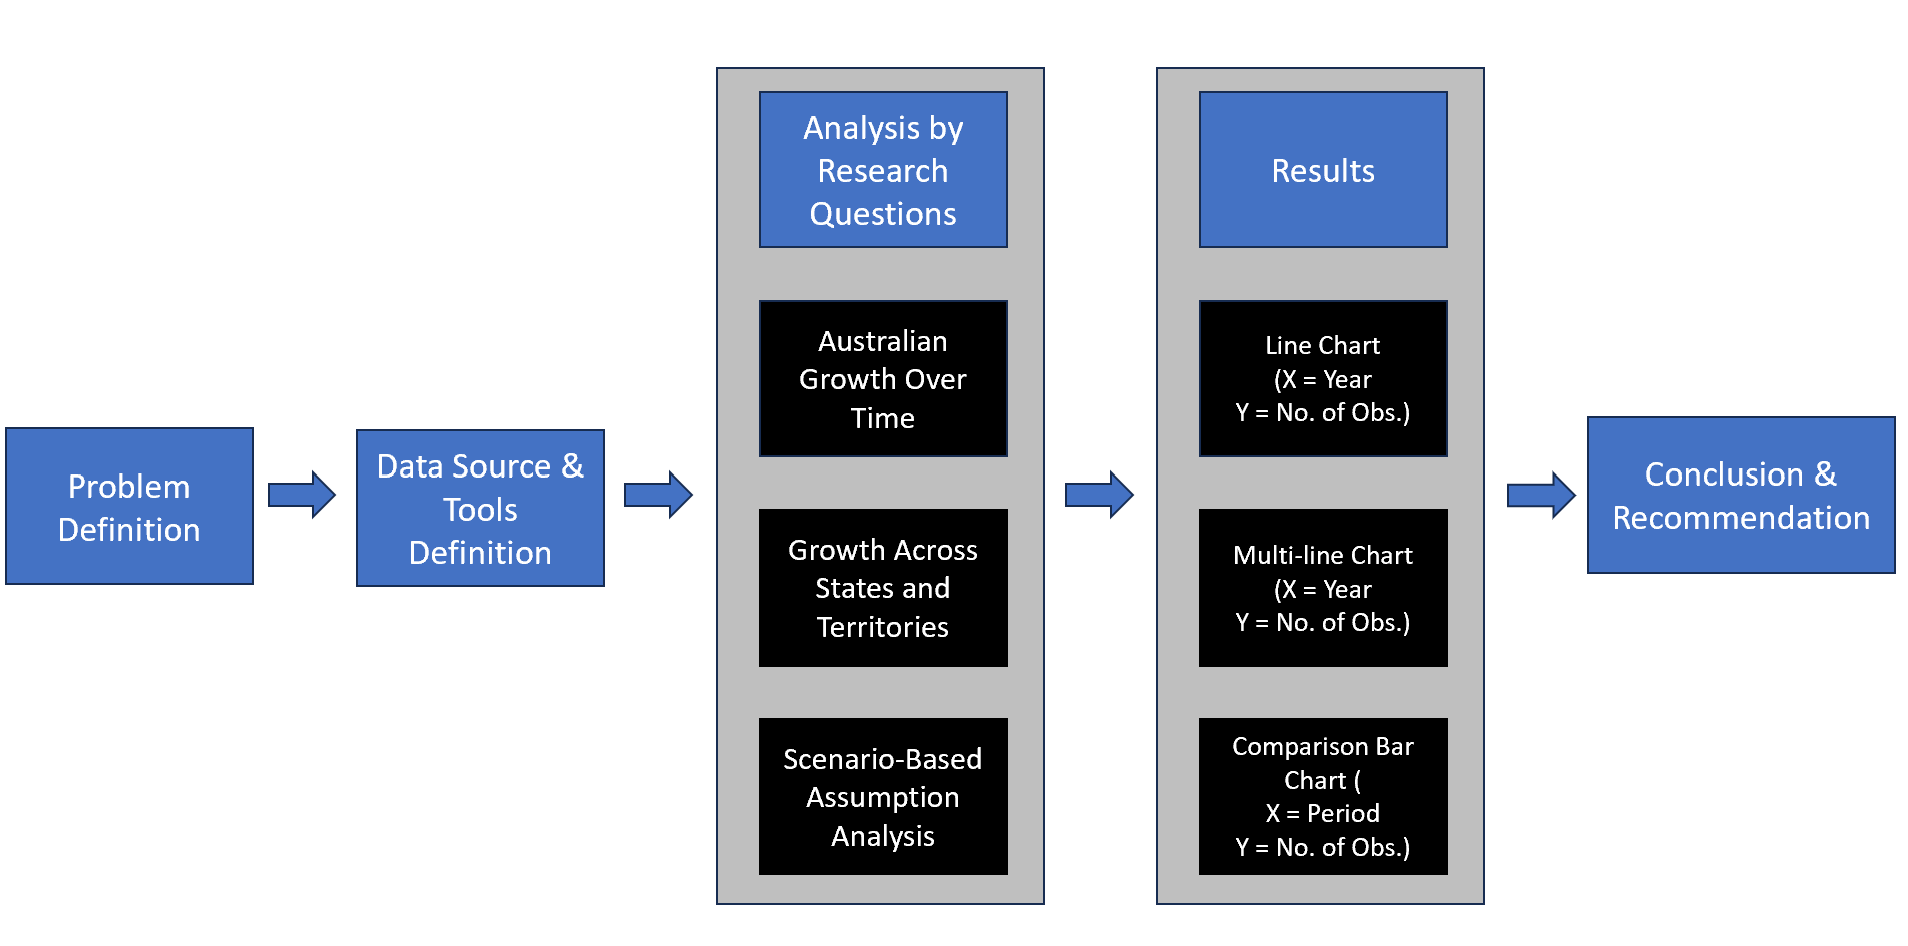
\includegraphics[keepaspectratio]{figures/methodology.png}}

}

\end{figure}%

Based on Figure~\ref{fig-methodology}, the population projection
analysis follows a clear, step-by-step framework that connects problem
definition to results and recommendations. It begins with identifying
the key issue: understanding how Australia's population will change over
time under different scenarios. The study recognises that future
population levels are influenced by varying rates of fertility,
mortality, and migration.

The second step defines the data source and tools used. The analysis is
based on the ABS Population Projections dataset from 2017 to 2066. The
data includes regional breakdowns, assumption categories, and annual
population figures. Tools such as R and libraries like tidyverse are
used for cleaning, aggregation, and visualisation.

The core analysis is guided by three research questions: How will
Australia's overall population grow? How will population trends differ
across states and territories? How do different demographic assumptions
impact these projections? Each of these questions forms a track of
analysis.

Results are presented using appropriate charts. National growth over
time is visualised with a line chart, showing how population changes
annually. State-level comparisons are made with a multi-line chart,
allowing direct comparisons between regions. For scenario-based
comparisons, a grouped bar chart is used. This chart compares the
average population in three periods---Start (2017--2033), Middle
(2034--2050), and End (2051--2066)---under three different assumptions:
Low, Medium, and High. The scenarios are defined based on combinations
of fertility rates, life expectancy, and migration levels.

Finally, the process leads to a conclusion and recommendation section,
where key findings are summarised and implications for planning are
discussed. This method ensures a logical flow from question to insight,
allowing policymakers and planners to interpret complex projection data
clearly.

\section{Data Description}\label{data-description}

\begin{tcolorbox}[enhanced jigsaw, rightrule=.15mm, colframe=quarto-callout-note-color-frame, opacitybacktitle=0.6, leftrule=.75mm, title=\textcolor{quarto-callout-note-color}{\faInfo}\hspace{0.5em}{Meta Data}, opacityback=0, toprule=.15mm, toptitle=1mm, breakable, colbacktitle=quarto-callout-note-color!10!white, bottomrule=.15mm, left=2mm, arc=.35mm, colback=white, coltitle=black, bottomtitle=1mm, titlerule=0mm]

\textbf{Title:} \emph{Australian Population Projections by Region
(2017--2066)}\\
\textbf{Description:} This dataset contains projected population
estimates for Australia's states and territories from 2017 to 2066 under
various demographic assumptions. Data was sourced from the Australian
Bureau of Statistics (ABS). Observations have been filtered, unnecessary
variables were removed and columns standardized to support regional
population trend analysis.\\
\textbf{Source:} Australian Bureau of Statistics --
\href{https://www.abs.gov.au}{abs.gov.au}\\
\textbf{Attribution:} © Commonwealth of Australia (ABS), accessed 30 May
2025.\\
\textbf{Time Coverage:} 2017--2066\\
\textbf{Geographic Scope:} All Australian states and territories\\
\textbf{Collected On:} 26 May 2025

\end{tcolorbox}

\subsection{Description of all
Variables}\label{description-of-all-variables}

\begin{longtable}[]{@{}
  >{\raggedright\arraybackslash}p{(\linewidth - 2\tabcolsep) * \real{0.5000}}
  >{\raggedright\arraybackslash}p{(\linewidth - 2\tabcolsep) * \real{0.5000}}@{}}
\caption{Description of variables in the Australian population
projection dataset}\label{tbl-vars}\tabularnewline
\toprule\noalign{}
\begin{minipage}[b]{\linewidth}\raggedright
\textbf{Variable}
\end{minipage} & \begin{minipage}[b]{\linewidth}\raggedright
\textbf{Description}
\end{minipage} \\
\midrule\noalign{}
\endfirsthead
\toprule\noalign{}
\begin{minipage}[b]{\linewidth}\raggedright
\textbf{Variable}
\end{minipage} & \begin{minipage}[b]{\linewidth}\raggedright
\textbf{Description}
\end{minipage} \\
\midrule\noalign{}
\endhead
\bottomrule\noalign{}
\endlastfoot
\texttt{Region} & Abbreviation for each Australian state or territory
(e.g., NSW, VIC, WA). \\
\texttt{Sex} & Sex category of the projection (e.g., ``Males'',
``Females''). \\
\texttt{Fertility\_Assumption} & Assumed fertility level used in
projection (e.g., ``Medium fertility''). \\
\texttt{Mortality\_Assumption} & Assumed mortality level used in
projection (e.g., ``Medium life expectancy''). \\
\texttt{NOM} & Numeric value of net overseas migration scenario. \\
\texttt{Overseas\_Migration} & Assumed level of net overseas migration
(e.g., ``Medium NOM''). \\
\texttt{NIM} & Numeric value of net interstate migration scenario. \\
\texttt{Interstate\_Migration} & Assumed level of net interstate
migration (e.g., ``Medium interstate flows''). \\
\texttt{Year} & Year of the population projection (2017 to 2066). \\
\texttt{Projected\_Population} & Estimated total population for the
specified region, year, and demographics. \\
\end{longtable}

Table~\ref{tbl-vars} shows a description of all the variables present in
the Australian Population Projections by Region (2017--2066) dataset
after cleaning.

\section{Results}\label{sec-results}

\subsection{Q1. How is Australia's total population projected to change
over the
years?}\label{q1.-how-is-australias-total-population-projected-to-change-over-the-years}

We applied the ``medium'' settings for fertility, mortality, and
migration to reflect the standard benchmark used in official planning.

\begin{figure}

\caption{\label{fig-total-projection}Projected population of Australia
from 2017 to 2066 under medium fertility, mortality, and migration
assumptions. Population is projected to rise to over 40 million by the
year 2066 indicating steady long-term growth.}

\centering{

\pandocbounded{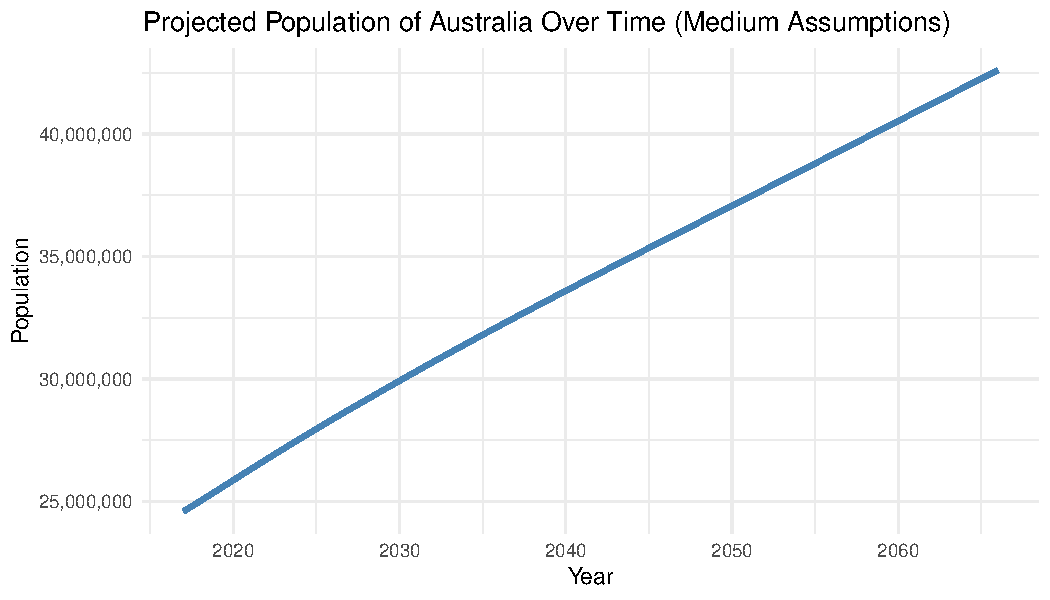
\includegraphics[keepaspectratio]{analysis_files/figure-pdf/fig-total-projection-1.pdf}}

}

\end{figure}%

Figure~\ref{fig-total-projection} shows a consistent upward trend in
Australia's population. Under medium demographic assumptions, the total
population is projected to grow steadily, reaching over 40 million by
2066.

\begin{figure}

\caption{\label{fig-growth-chart}Projected annual population growth rate
of Australia from 2017 to 2066 under medium fertility, mortality, and
migration assumptions. Growth rate is projected to decline to below 1\%
by 2066.}

\centering{

\pandocbounded{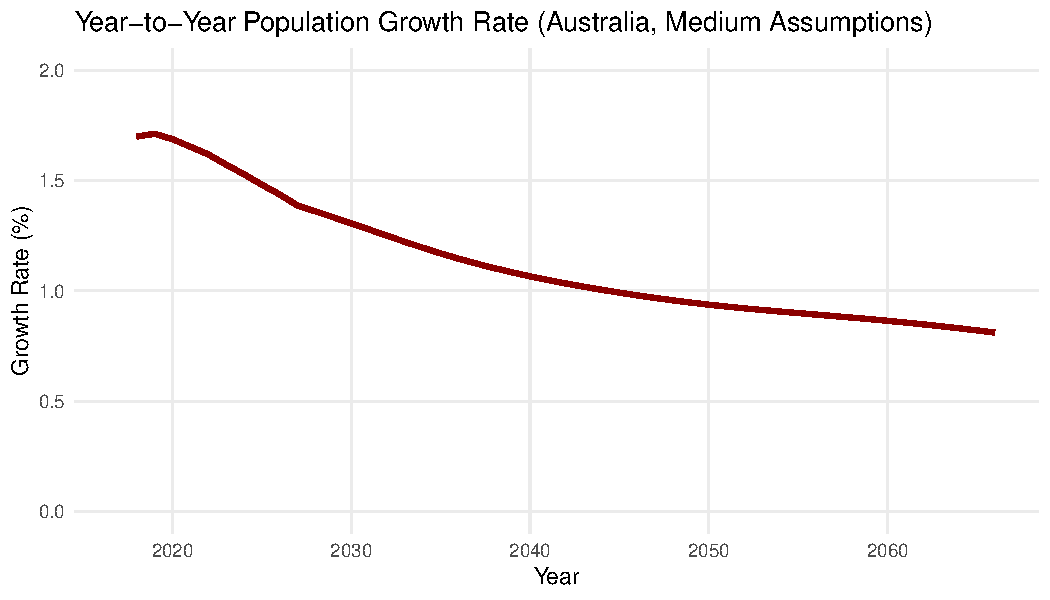
\includegraphics[keepaspectratio]{analysis_files/figure-pdf/fig-growth-chart-1.pdf}}

}

\end{figure}%

Figure~\ref{fig-growth-chart} shows that while the population grows, the
annual growth rate slows over time, falling below 1\% by 2066. This
suggests a gradual deceleration in population increase despite overall
growth.

\subsection{Q2. How is the total population projected to grow across
different states and territories over
time?}\label{q2.-how-is-the-total-population-projected-to-grow-across-different-states-and-territories-over-time}

\begin{figure}

\caption{\label{fig-regional-chart}Indexed population growth in
Australia by region from 2017 to 2066 under medium fertility, mortality,
and migration assumptions. Each region's population is set to 100 in
2017 to compare relative growth.}

\centering{

\pandocbounded{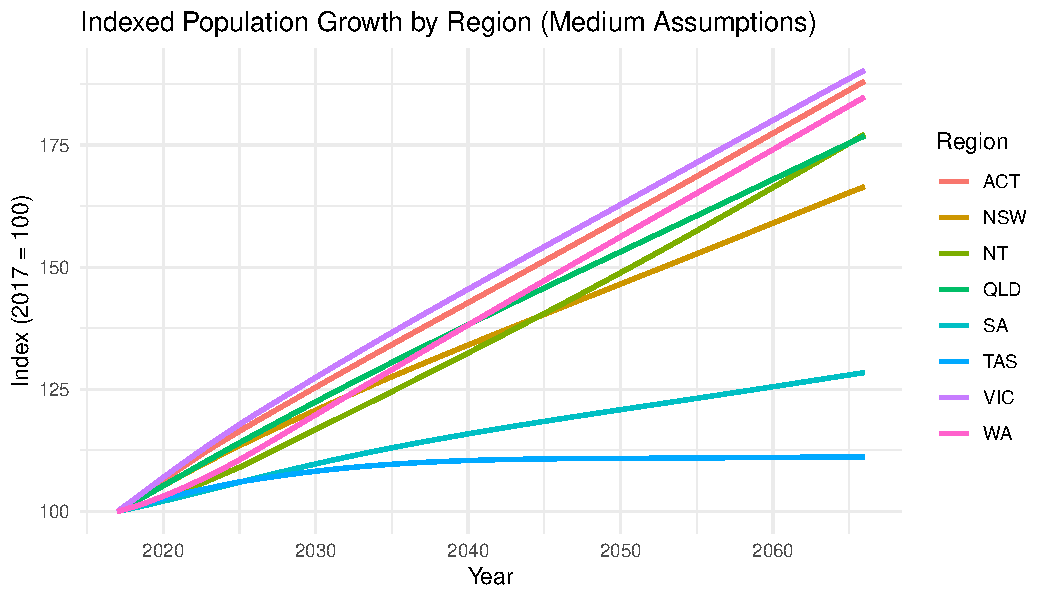
\includegraphics[keepaspectratio]{analysis_files/figure-pdf/fig-regional-chart-1.pdf}}

}

\end{figure}%

Figure~\ref{fig-regional-chart} highlights clear variation across
regions. Population growth is fastest in Queensland, Victoria, and New
South Wales, while Tasmania and South Australia show slower increases.
This suggests uneven demographic pressures and different infrastructure
needs across the country.

\subsection{Q3. How do different assumptions (fertility, mortality,
migration) influence these
projections?}\label{q3.-how-do-different-assumptions-fertility-mortality-migration-influence-these-projections}

\begin{figure}

\caption{\label{fig-assumption-scenario}Projected population of
Australia from 2017 to 2066 under medium fertility, mortality, and
migration assumptions. The High scenario consistently projects the
largest population, driven by higher fertility and migration, while the
Low scenario shows slower growth due to reduced births and zero net
migration.}

\centering{

\pandocbounded{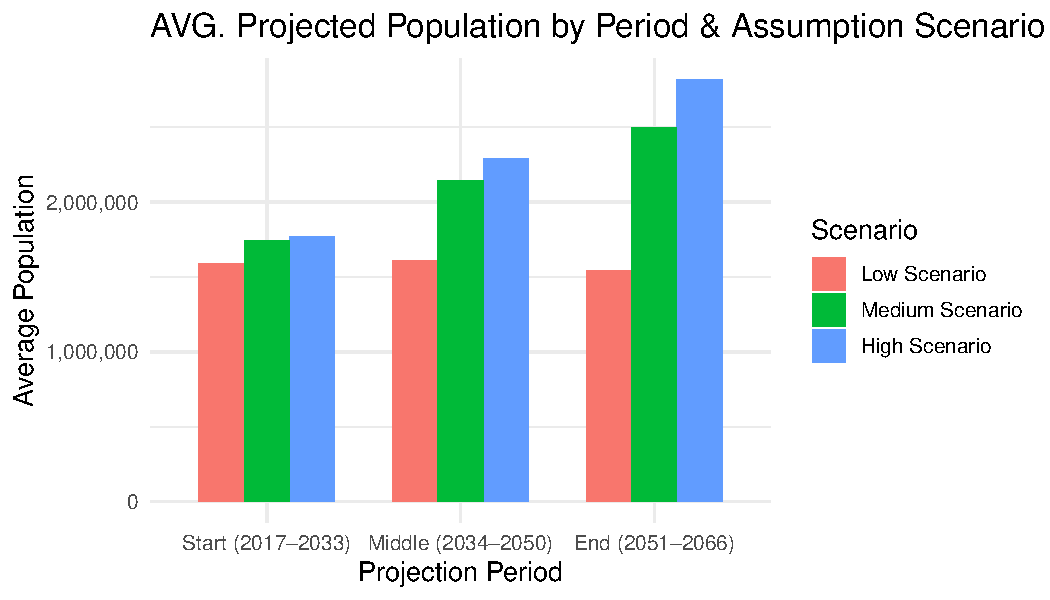
\includegraphics[keepaspectratio]{analysis_files/figure-pdf/fig-assumption-scenario-1.pdf}}

}

\end{figure}%

Figure~\ref{fig-assumption-scenario} compares three demographic
scenarios. While all scenarios begin similarly, projections diverge over
time. The High scenario leads to the largest population by 2066, driven
by higher fertility and migration. In contrast, the Low scenario results
in slower growth, showing the strong influence of policy and global
trends on long-term outcomes.

\section{Discussion, Conclusion and
Recommendation}\label{discussion-conclusion-and-recommendation}

\subsection{Discussion}\label{discussion}

The population projection analysis underscores a crucial insight:
Australia is poised for sustained population growth, but the pace and
distribution of this growth are highly variable depending on regional
and demographic factors. Nationally, the population is expected to
surpass 40 million by 2066 under medium assumptions, showing steady
long-term growth. However, the annual growth rate is projected to
decline gradually, falling below 1\% by the projection's end. Regional
differences are prominent, with faster growth in Victoria, New South
Wales, and Queensland, while smaller states experience slower increases.
Moreover, varying assumptions about fertility, mortality, and migration
create distinct population futures, highlighting the significant impact
of policy and social trends on Australia's demographic trajectory.

The population projection analysis underscores a crucial insight:
Australia is poised for sustained population growth, but the pace and
distribution of this growth are highly variable depending on regional
and demographic factors.

Firstly, the national upward trend in population is consistent across
all assumption scenarios, though the growth rate slows over time,
dropping below 1\% by 2066. This tapering growth may reflect demographic
maturity, where lower fertility rates and aging populations contribute
to deceleration despite net migration.

Secondly, state and territory-level comparisons reveal stark differences
in regional population trajectories. Victoria has consistently
maintained the leading position in terms of indexed growth under medium
assumptions, reflecting its enduring strength as both an economic hub
and a major destination for internal and international migration.
However, from 2030 onwards, Western Australia shows a notable
acceleration in growth, indicating its rising prominence as an emerging
economic and migration magnet. In contrast, states like Tasmania and
South Australia continue to experience comparatively slower growth,
which may pose challenges in sustaining economic vitality and public
service provision amid relatively stagnant populations. These regional
disparities highlight the importance of implementing place-based
planning strategies tailored to the distinct demographic and economic
contexts of each state.

Thirdly, the influence of demographic assumptions is significant. The
differences between low, medium, and high scenarios amplify as
projections move further into the future. This sensitivity analysis
shows that migration policies and fertility trends are pivotal levers
that can drastically alter Australia's demographic future. For instance,
a high-migration, high-fertility scenario leads to a considerably larger
population by 2066 than a conservative one. This raises questions about
the country's infrastructure readiness, environmental sustainability,
and social cohesion under varying scenarios.

\subsection{Conclusion}\label{conclusion}

Australia's population is projected to grow significantly over the next
five decades, but this growth will not be evenly spread across regions
nor equally influenced by demographic factors. Nationally, the
population is on track to exceed 40 million by 2066 under medium
assumptions, though regional growth will be uneven.

The study confirms three major takeaways:

\begin{enumerate}
\def\labelenumi{\arabic{enumi}.}
\item
  Sustained national growth---but at a declining rate.
\item
  Regional disparities in growth, with populous and economically active
  states growing faster.
\item
  Critical dependency on assumptions---particularly fertility and
  migration rates---that shape long-term projections.
\end{enumerate}

These findings carry profound implications for urban planning, public
service delivery, environmental resource management, and economic
development strategies.

\subsection{Recommendation}\label{recommendation}

\begin{enumerate}
\def\labelenumi{\arabic{enumi}.}
\item
  Targeted regional strategies: Regional differences call for
  differentiated planning. States like Tasmania and South Australia
  might need economic incentives or migration programs to stimulate
  growth, while high-growth areas like Victoria should prioritize
  housing, transport, and social infrastructure to prevent strain.
\item
  Demographic monitoring \& Policy adjustments: Real-time demographic
  data (fertility, migration trends, mortality) must be monitored
  closely. Adjustments to immigration quotas, family support policies,
  and healthcare planning can help steer population growth toward
  sustainable and desirable outcomes.
\item
  Policy-makers need to challenge projection assumptions: Are fertility
  rates likely to change due to policy or social shifts? Could
  unexpected migration events (e.g.~geopolitical crises) alter
  projections? Besides, they should use comparative frameworks from
  other nations experiencing similar demographic transitions (e.g.,
  Canada, the UK) to benchmark potential outcomes.
\item
  Further research recommended includes:
\end{enumerate}

\begin{itemize}
\item
  Investigate the implications of population aging in slower-growing
  states.
\item
  Model how external shocks (e.g.~pandemics, climate migration) might
  impact current projections.
\item
  Study correlations between population growth and environmental impact
  at a regional level.
\end{itemize}

\section{Reference}\label{reference}

Australian Bureau of Statistics. (2023). Population Projections,
Australia, 2017 to 2066\,(Data Explorer Table). Retrieved May 2025,
\href{https://dataexplorer.abs.gov.au/vis?tm=Population\%20Projections&pg=0&hc\%5BPeople\%5D=Population\%20\%3E\%20Population\%20Projections&df\%5Bds\%5D=PEOPLE_TOPICS&df\%5Bid\%5D=POP_PROJ_REGION_2012_2061&df\%5Bag\%5D=ABS&df\%5Bvs\%5D=1.0.0&pd=2017\%2C&dq=1\%2B2\%2B3\%2B4\%2B5\%2B6\%2B7\%2B8.1\%2B2.TT.1\%2B2\%2B3.1.1\%2B2\%2B3\%2B4.1\%2B2\%2B3.A&ly\%5Bcl\%5D=SEX_ABS&ly\%5Brs\%5D=FERTILITY\%2CNOM\%2CNIM&ly\%5Brw\%5D=TIME_PERIOD\%2CREGION&to\%5BTIME_PERIOD\%5D=false&vw=ov}{Access
data here}

Wickham, H. (2016). ggplot2: Elegant graphics for data analysis.
Springer-Verlag New York. \url{https://ggplot2-book.org}

Xie Y (2024). \emph{knitr: A General-Purpose Package for Dynamic Report
Generation in R}. R package version 1.49,
\url{https://yihui.org/knitr/}.

Wickham H, Averick M, Bryan J, Chang W, McGowan LD, François R,
Grolemund G, Hayes A, Henry L, Hester J, Kuhn M, Pedersen TL, Miller E,
Bache SM, Müller K, Ooms J, Robinson D, Seidel DP, Spinu V, Takahashi K,
Vaughan D, Wilke C, Woo K, Yutani H (2019). ``Welcome to the
tidyverse.'' \emph{Journal of Open Source Software}, \emph{4}(43), 1686.
doi:10.21105/joss.01686 \url{https://doi.org/10.21105/joss.01686}.




\end{document}
